\documentclass{article}   

\usepackage{geometry}
\usepackage{qtree}
\usepackage[square,numbers]{natbib}
% \usepackage{cite}  
\geometry{a4paper}

\usepackage[]{algorithm2e}
\usepackage{amsthm}
\newtheorem{theorem}{Theorem}[section]
\newtheorem{corollary}{Corollary}[theorem]
\newtheorem{lemma}[theorem]{Lemma}
\usepackage{rotating}
\usepackage[utf8]{inputenc}
\usepackage[T1]{fontenc}    % use 8-bit T1 fonts
\usepackage{lmodern}
\usepackage{hyperref}       % hyperlinks
\usepackage{lipsum}

\usepackage{color, colortbl}

\definecolor{Gray}{gray}{0.9}

\usepackage[protrusion=true,expansion=true]{microtype}

\usepackage{amssymb}
\usepackage{amsfonts}
\usepackage{eqnarray,amsmath}
\usepackage[table]{xcolor}

\usepackage{listings}
\usepackage{graphicx}
\usepackage{dirtytalk}

\usepackage{rotating}
\usepackage{caption}

%% if you use PostScript figures in your article
%% use the graphics package for simple commands
\usepackage{graphics}


%% or use the graphicx package for more complicated commands
\usepackage{graphicx}
\usepackage[table]{xcolor}

\usepackage{indentfirst}
\usepackage[utf8]{inputenc}
 \usepackage{subcaption}
\usepackage{xcolor}
 
\usepackage{xspace,color}
\usepackage{url}



\lstset{commentstyle=\color{red},keywordstyle=\color{black},
showstringspaces=false}
\lstnewenvironment{rc}[1][]{\lstset{language=R}}{}
\newcommand{\ri}[1]{\lstinline{#1}}  %% Short for 'R inline'

\lstset{language=R}             % Set R to default language


%https://tex.stackexchange.com/questions/96825/nicely-formatted-where-statement-for-maths
 \newenvironment{where}{\noindent{}where\begin{itemize}}{\end{itemize}}
 \renewcommand*\descriptionlabel[1]{\hspace\leftmargin$#1$}
 
\lstset{escapeinside={<@}{@>}}
% please place your own definitions here and don't use \def but
% \newcommand{}{}
%
% Insert the name of "your journal" with
% \journalname{myjournal}
%
\begin{document}

\title{%
  Practice 8: Bayesian Theorem} %\\~\\
  %\Large }
\author{Mayra Cristina Berrones Reyes 6291}

\maketitle

\section{Introduction}

In this work, we will discuss a lot about the bayesian theorem, specifically aimed to review some of the information available to the general public, and some to data enthusiast, about the current COVID-19 pandemic. \\

Before we begin with the discussion of some of the links shared in class, and associated information within, it is very important to remark on some of the subjects that we are going to be using recurrently along this work, and that is the use of appropriate metrics to rate the results of the experiment at hand.\\

Figure \ref{fig1} shows the confusion matrix for each of the classical metrics. In all cases, TP (True positives) represents if the result of the test is positive, and the patient actually has COVID. The same applies to TN (True negatives) in which, the test turns out negative, so the patient is healthy. FP (False positives) are the cases when the patient is healthy and the test says he has COVID. FN (False negatives) are when the test shows no sign of the disease, but the patient has it \cite{mitesis}.\\

\begin{figure}[]
\begin{subfigure}{.24\textwidth}
  \centering
  \includegraphics[width=.9\linewidth]{accuracy.png}  
  \caption{  }
  \label{sb1-1}
\end{subfigure}
\begin{subfigure}{.24\textwidth}
  \centering
  \includegraphics[width=.9\linewidth]{presision.png}  
  \caption{ }
  \label{sb1-2}
\end{subfigure}
\begin{subfigure}{.24\textwidth}
  \centering
  \includegraphics[width=.9\linewidth]{recall.png}  
  \caption{ }
  \label{sb1-3}
\end{subfigure}
\begin{subfigure}{.24\textwidth}
  \centering
  \includegraphics[width=.9\linewidth]{sensitivity.png}  
  \caption{ }
  \label{sb1-4}
\end{subfigure}
	\caption{This figure represents the confusion matrix for: a) Accuracy, b) Precision, c) Recall or Sensitivity, and d) Specificity. In each confusion matrix, the colored boxes represent the features in which the metrics relay more heavily.}
\label{fig1}
\end{figure}

The first metric we have is the accuracy, which confusion matrix is depicted as a) in Figure \ref{fig1}. It computes the percentage of correct predictions over all kinds of predictions made, see Equation (\ref{eq2}). This is a good indicator of performance when the data we have is balanced. In our case, if the number of cases positive with COVID and without them is nearly the same.\\

\begin{eqnarray}
\label{eq2}
\text{Accuracy} = \frac{TP + TN}{TP + FP + FN + TN}		
\end{eqnarray}

The next metric is precision (Equation (\ref{eq3})) which computes the proportion of positive predictions being positive. It tells us about the success probability of making a correct positive test.\\

\begin{eqnarray}
\label{eq3}
\text{Precision} = \frac{TP}{TP + FP}		
\end{eqnarray}

The recall, Equation (\ref{eq4}), explains how sensitive the model is towards identifying the positive class of the tests. It is the proportion of true positives cases that were classified as positive, it is also known as the true positive rate.\\

\begin{eqnarray}
\label{eq4}
\text{Recall} = \frac{TP}{TP + FN}		
\end{eqnarray}

Specificity, Equation (\ref{eq6}), is the opposite of Recall and focuses on the proportion of the negative cases that were classified as negative by the network; thus, it is a measure of how well the classifier identifies negative cases. It is also known as the true negative rate.

\begin{eqnarray}
\label{eq6}
\text{Specificity} = \frac{TN}{TN + FP}		
\end{eqnarray}

Lastly, we have the F1 score.This metric combines precision and recall relative to a specific positive class, as seen in Equation (\ref{eq5}). The F1 score can be seen as a weighted average of the precision and recall, where an F1 score reaches its best value at 1 and worst at 0.\\
\begin{eqnarray}
\label{eq5}
\text{F1 Score} = \frac{2 \cdot \text{Precision} \cdot \text{Recall}}{(\text{Precision} + \text{Recall})}		
\end{eqnarray}

\section{Preliminary discussion}

Now that we are clear about the different metrics used to evaluate the results, we begin the discussion of the multiple links shared in class. Without going in a specific order, this articles show some very interesting information about how we interpret test results from COVID-19, and introduces the highly important notion that the current way of testing and gathering results, may not be the optimal solution to accurately portray the behavior of the virus.\\

Testing for COVID is a privilege not many country have, and even in places where they are available, they are scarce, and not accessible enough for the general public because of the pricing. The present way of testing for COVID is shown in Table \ref{tab1}.\\

\begin{table}[]\caption{COVID testing basic information.}
\label{tab1}
\begin{tabular}{|p{2.7cm}|p{3.4cm}|p{3.4cm}|p{3.4cm}|}
\hline
     & Molecular test & Antigen test & Antibody test \\
\hline
Also known as: & Diagnostic test, RT-PCR& Rapid diagnostic test& Serological test, blood test\\
\hline
How is taken: & Nasal or throat swab, saliva&Nasal or throat swab& Finger stick or blood draw\\
\hline
Is another test needed: & This test is usually highly accurate and usually does not need repeat&Positive results are highly accurate. May need confirmation of molecular test.&Sometimes a second antibody test is required\\
\hline
What it shows: & Diagnosis active COVID infection & Diagnosis active COVID infection& shows if you have been infected by COVID in the past\\
\hline
What it does \textbf{not} do: & Show if you ever had COVID or were infected in the past. & Definitively rule out active COVID infection. Antigen test are more likely to miss an active virus infection compared to molecular tests.& Diagnose active COVID infection at the time of the test, or show that you do not have COVID\\
\hline
\end{tabular}
\end{table}


In this case, the standard reference for the diagnosis of COVID are the RT-PCR or molecular tests. As shown in Table \ref{tab1} they have better accuracy than the other two. The alternative tests to this are the Antigen test, and antibody test. Both of this test have fairly accurate positive results, but if they come back negative, the general recommendation is to have a molecular test done.\\

Both molecular and antigen tests are diagnostic tests, which means that they show in their results if you have an active infection of COVID. The difference between the two is that the molecular test help to detect the genetic material of the virus, whilst the antigen tests detect specific proteins on the surface of the virus \cite{fda1}.\\

So what does that mean for the regular folk? It means that generally speaking, the antigen test can give a faster diagnostic on an active infection of COVID than a molecular test, but they have a higher probability of having a false negative.\\ 

Same goes with the antibody tests. They offer a fast and cheaper version of the test, but it should not be used to diagnose an active infection, since they only can detect if our immune system has developed antibodies to fight the virus, not the virus itself. This is tricky, because the human body takes up several weeks to develop enough antibodies to be detected in this test. If one is a target person for COVID, they may not have the luxury of waiting a few weeks to see their results.\\

With all of this instances we are presented with another point of view in regard of the result of the test and their reliability. In M\'exico it is common to find the mentality of, do not fix it if it is not broken, so when it comes to health, many of the people testing for COVID are likely to have shown symptoms before going to the hospital. Some of the articles presented in class mention the notion of pre-test probability, which encircle the cases that are more likely or less likely to show positive results on a COVID test, comparing between cases of people highly exposed to the virus, versus people that respected quarantine, but still show symptoms.\\

As for the probability that the test are reliable, some articles mention that the sensitivity of the molecular test is of 63\%, and in the case of antigen test is 31\% for detecting an active infection. As stated before, an antibody test does not test active infections, but in order to be effective, the patient has to wait at least a week before the symptoms to perform this test, and up to 15 days, for it to perform optimally. It makes an excellent test to have post disease because it shows if your body is correctly fighting the virus, and in time could give us pointers in case of a new outbreak \cite{chan2020}.\\

Because this last test is too dependent on time and various others factors, it is hard to find a source that tells us with certainty the percentage of reliability of this test. Performed after the 15 days or more after the symptoms, the accuracy can go from 75 to 90 percent \cite{cont}.\\

In all this cases they use the bayesian theorem to revise the result of probability that a test may show in the results. The metric used generally is the sensitivity or recall. \\

\section{Experimentation}

For the experimentation in this work, we took a data base from Kaggle \cite{kaggle}, that represents the cases reported in Mexico up to the month of October of 2020. \\

\begin{figure}[]
\begin{subfigure}{.5\textwidth}
  \centering
  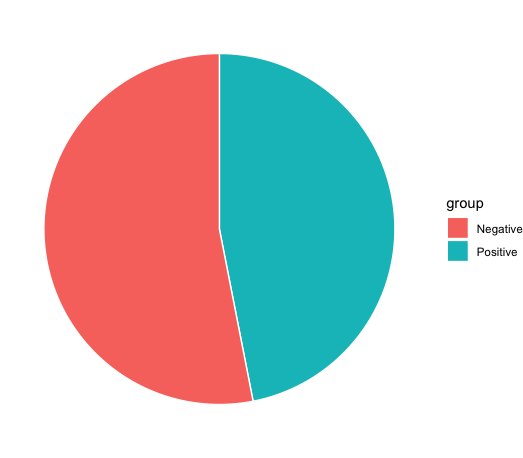
\includegraphics[width=1\linewidth]{ej8_pie2.png}  
  \caption{  }
  \label{sb2-1}
\end{subfigure}
\begin{subfigure}{.5\textwidth}
  \centering
  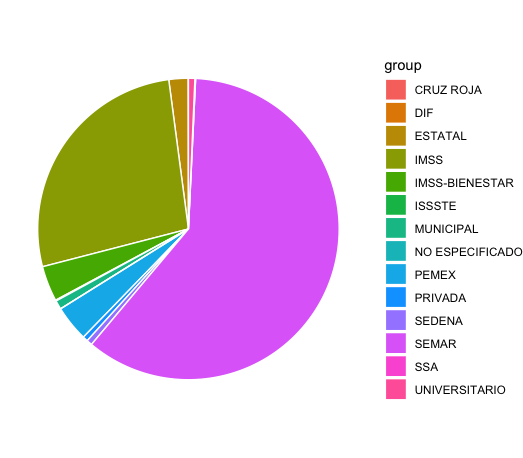
\includegraphics[width=1\linewidth]{ej8_pie.png}  
  \caption{ }
  \label{sb2-2}
\end{subfigure}
	\caption{Total of positive and negative cases in Mexico (a) and distribution of all cases in different health institutions (b).}
\label{fig2}
\end{figure}

Using some of the columns in the file, in Figure \ref{sb2-1} we can appreciate a plot with the distribution of all positive and negative tests results, and on Figure \ref{sb2-2} the distribution of the total of cases in each hospital institution. The hospital plot helped us with the investigation of the COVID tests permitted in Mexico. \\

The two we found some information of were the Architect SARS CoV-2 IgG of Abbot Laboratories Inc \cite{xalaka}, with a sensitivity of 95.8\% and specificity of 99\% \cite{fda2}. This is the more expensive one, and as far as we could search, not available in Tamaulipas (state where we researched more because of personal reasons). The other, more available is the MAGLUMI 2019-nCoV IgG (CLIA) of Shenzhen New Industries Biomedical Engineering \cite{xalaka} with 69.9\% on sensitivity and 97.5\% of specificity \cite{fda2}. \\ 
 
 In the case of antibody tests, we could not find the right one, because they are done in private labs, since is blood work. The only thing we could find was its price, and it rounds between 1,000 and 2,000 Mexican pesos, depending on the urgency of the results and the laboratory it is made on (Again, this information could be only be verified in Tamaulipas).\\
 
 Taking into consideration the experiment made in one of the links shared in class \cite{tds} we could replicate the procedure, using the data we could gather from the data set, and the reliability of the tests found.\\
 
 According to our data set, we have 370,713 positive cases and 419,350 negative cases of all tested subjects. In total we have 790,063 tests. Giving this data the probability of specificity and sensibility of the Architect SARS CoV-2 IgG, we have the results of Table\ref{tab2}.\\
 
 \begin{table}[]\caption{Table of predictions for the Architect SARS CoV-2 IgG test.}\label{tab2}
\centering
\begin{tabular}{| l | c | c |}
\hline
 & 1 & 0\\
\hline 
1&355,144 &15,570\\
\hline 
0&4,194&415,157\\
\hline
\end{tabular}
\end{table}


\begin{itemize}
\item Accuracy: 0.9749
\item Precision: 0.9580
\item Sensitivity: 0.9883
\item Specificity: 0.9638
\end{itemize}

Then we have the Bayes theorem:\\
\begin{equation}
\label{eq:bayes}
\begin{split}
P(A \mid B)& =\frac{ P(A) P(B \mid A)} { (P(A)P(B\mid A) + P(not A) P(B \mid not A))}\\~\\
&= \frac{0.454822 * 0.958}{(0.454822 * 0.958) + (0.545178 * 0.042)}\\~\\
&=\frac{0.4357195}{0.458017}=0.95007
\end{split}
\end{equation}


Following the experiment, we calculate the other metrics with the information from Table \ref{tab3} for the MAGLUMI 2019-nCoV IgG (CLIA) test.\\

 \begin{table}[]\caption{Table of predictions for the MAGLUMI 2019-nCoV IgG (CLIA) test.}\label{tab3}
\centering
\begin{tabular}{| l | c | c |}
\hline
 & 1 & 0\\
\hline 
1&259,128 &111,584\\
\hline 
0&10,483&408,866\\
\hline
\end{tabular}
\end{table}

\begin{itemize}
\item Accuracy: 0.8454
\item Precision: 0.6990
\item Sensitivity: 0.9611
\item Specificity: 0.7856
\end{itemize}


Then we have the Bayes theorem for the second test:\\
\begin{equation}
\label{eq:bayes2}
\begin{split}
P(A \mid B)& =\frac{ P(A) P(B \mid A)} { (P(A)P(B\mid A) + P(not A) P(B \mid not A))}\\~\\
&= \frac{0.341252533* 0.6990}{(0.341252533* 0.6990) + (0.658747467 * 0.3010)}\\~\\
&=\frac{0.2385355206}{0.4368185082}=0.54607466
\end{split}
\end{equation}


After this experiments we can clearly see the difference in reliability on both tests. In the Architect SARS CoV-2 IgG test, if we test positive, there is a probability of 95\% that we have COVID. In change, with the MAGLUMI 2019-nCoV IgG (CLIA) test, if we test positive, there is a 54\% probability that that diagnosis is correct. \\

\section{Conclusions}

The results of both experiments match the description that we had in mind, because we asked a health professional about the difference in testing, and, although he did not know the exact probability, the numbers are close enough to what he told us where the accuracy of the test. \\

In Tamaulipas, the standard way of testing is via antibodies if you are not a person in risk (Age, pre existing conditions, pregnant, etc) because in public hospitals, such as the IMSSS, ISSSTE, IPSET, etc., they have a very limited amount of testing material. The expert we contacted for information, can verify that they only have kits for rapid testing, so their results would be more like the MAGLUMI 2019-nCoV IgG (CLIA) test.\\

This work can help highlight the importance of having better testing equipment, since we are approaching the time of year when influenza and flu cases arise, as well as cases of dengue, because of all the rains of following months. Hospitals will be once again overflowed with people worried that they may be sick from COVID, and with test with poor reliability, resources like respirators and medicine, will become scarce again from diseases that may not even be COVID.\\

As a final thought, this work helped clear some things about COVID. In all the investigation we stumbled on, we found out that getting sick and recover does not mean that you are immune now (contrary to what some foreign president may say). And although it was quite an extensive work comparing sources and fishing everywhere for some information, I am glad that in most of the easy to find data does not have alarming head lines like, testing for COVID is unreliable. \\

If nothing else, this will help me explain to my family why and what is useful information about COVID, so they do not believe every gossip they pass on group chats.\\

\section{Extras}

Since we began experimenting a little bit with R and data mining (Python was the preferred method) we made two plots that did not quite fit with the rest of the experimentation, but they showed some important information. For example, in Figure \ref{fig3} we see the distribution of positive cases of COVID.\\

In Figure \ref{fig:LandscapeFigure} we were curious about the new information in the news, that not only older people were at risk of contracting COVID. We made an histogram with intervals of ages, and found that the most recurrent age of positive cases lies in the interval of 30 to 40 years old. This of course can be because that is the demographic that is more likely to have to go to work, and thus has more chances of getting infected.\\

\begin{figure}[]
  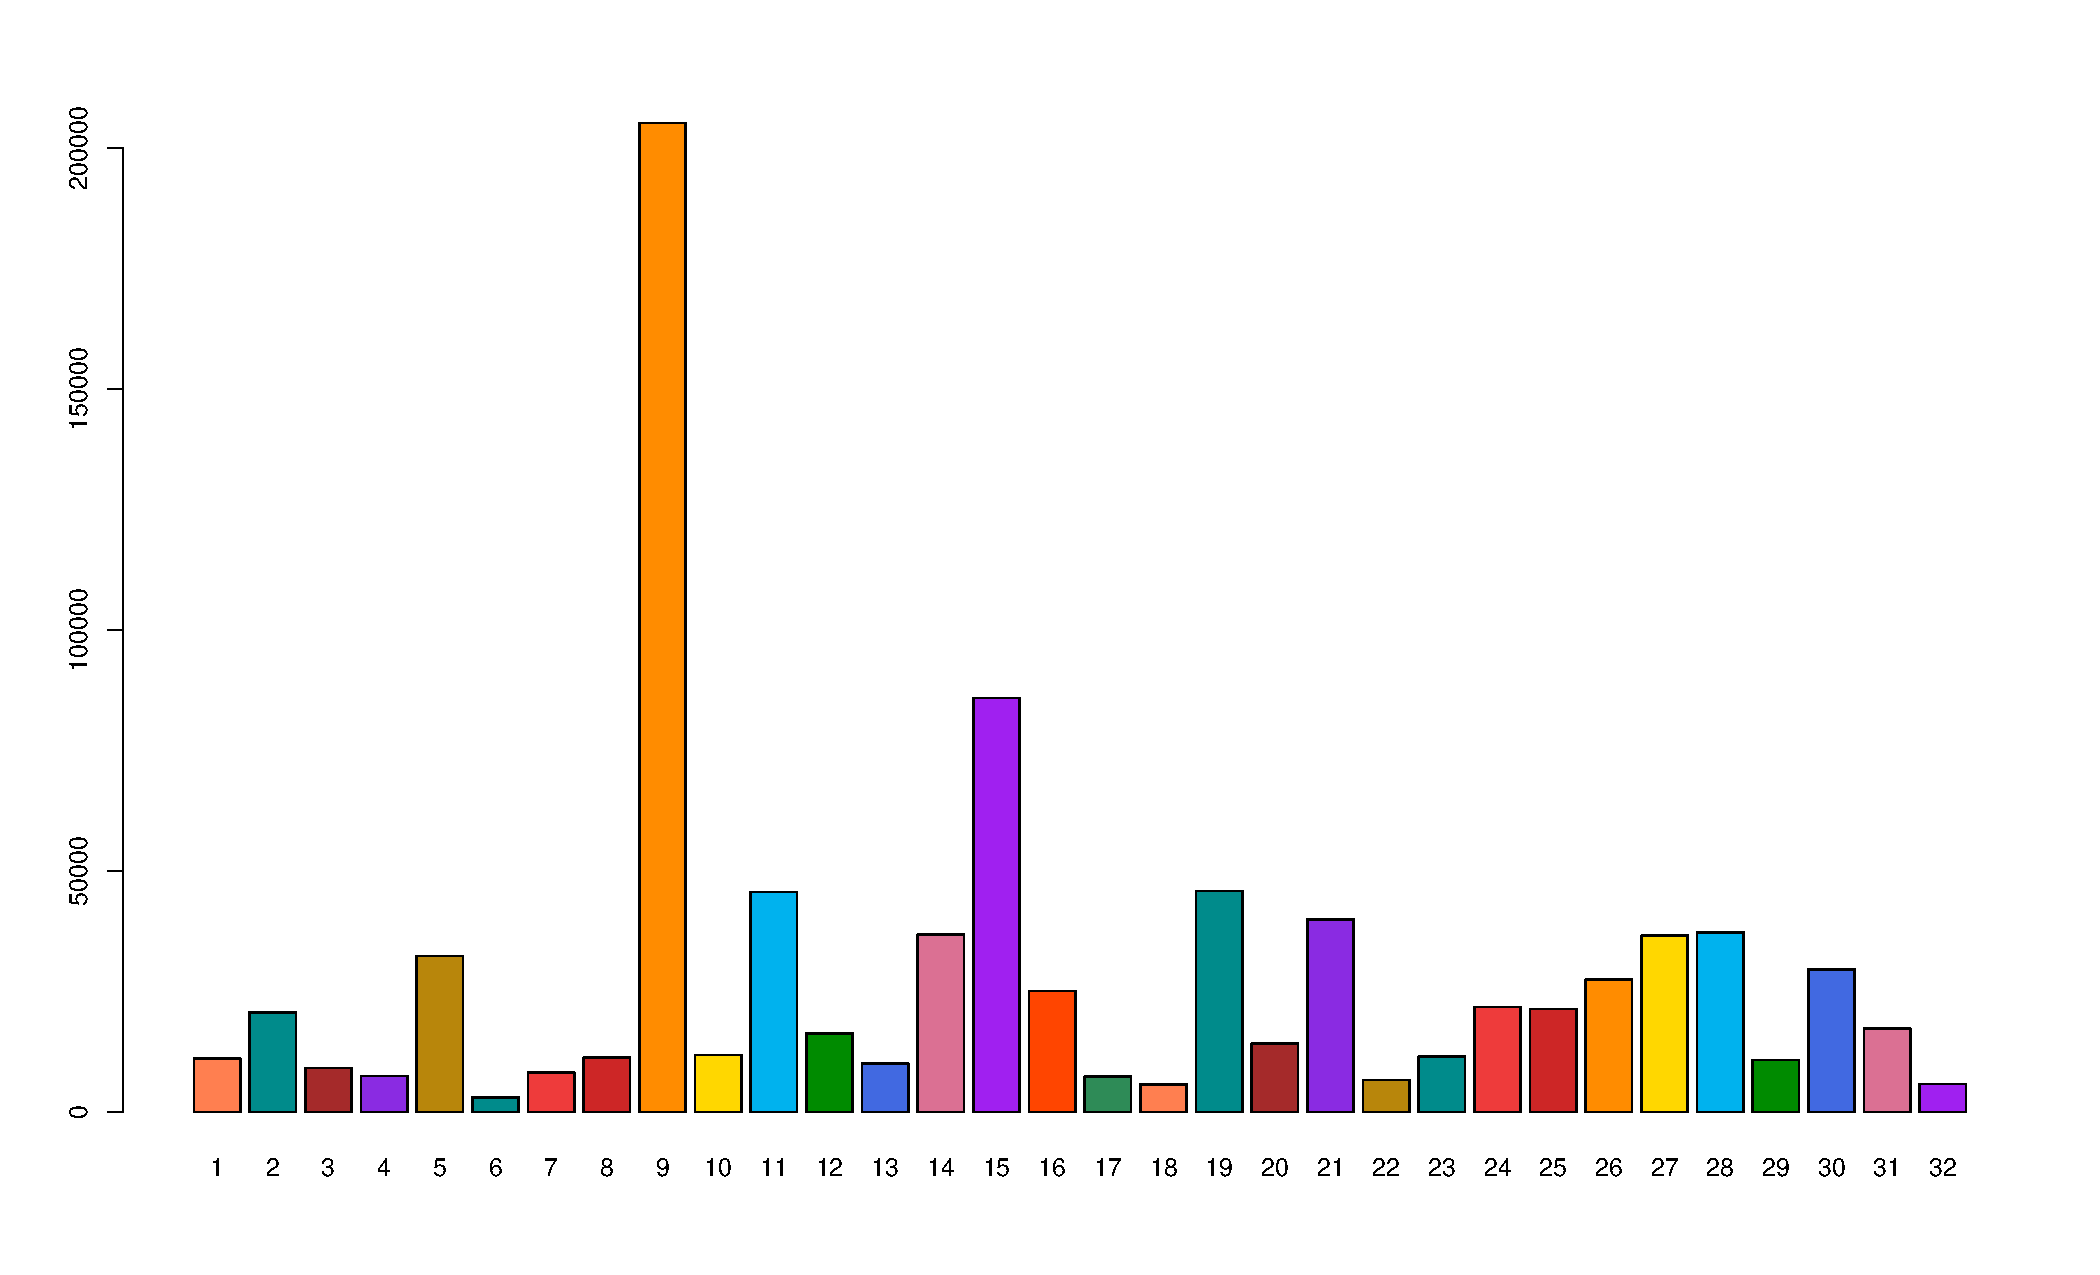
\includegraphics[width=1\linewidth]{Rplot01.pdf}  
	\caption{This plot represents all of the states in Mexico, and the total of cases reported in each one. The number represents a different federative state.}
\label{fig3}
\end{figure}


\begin{sidewaysfigure}[]
    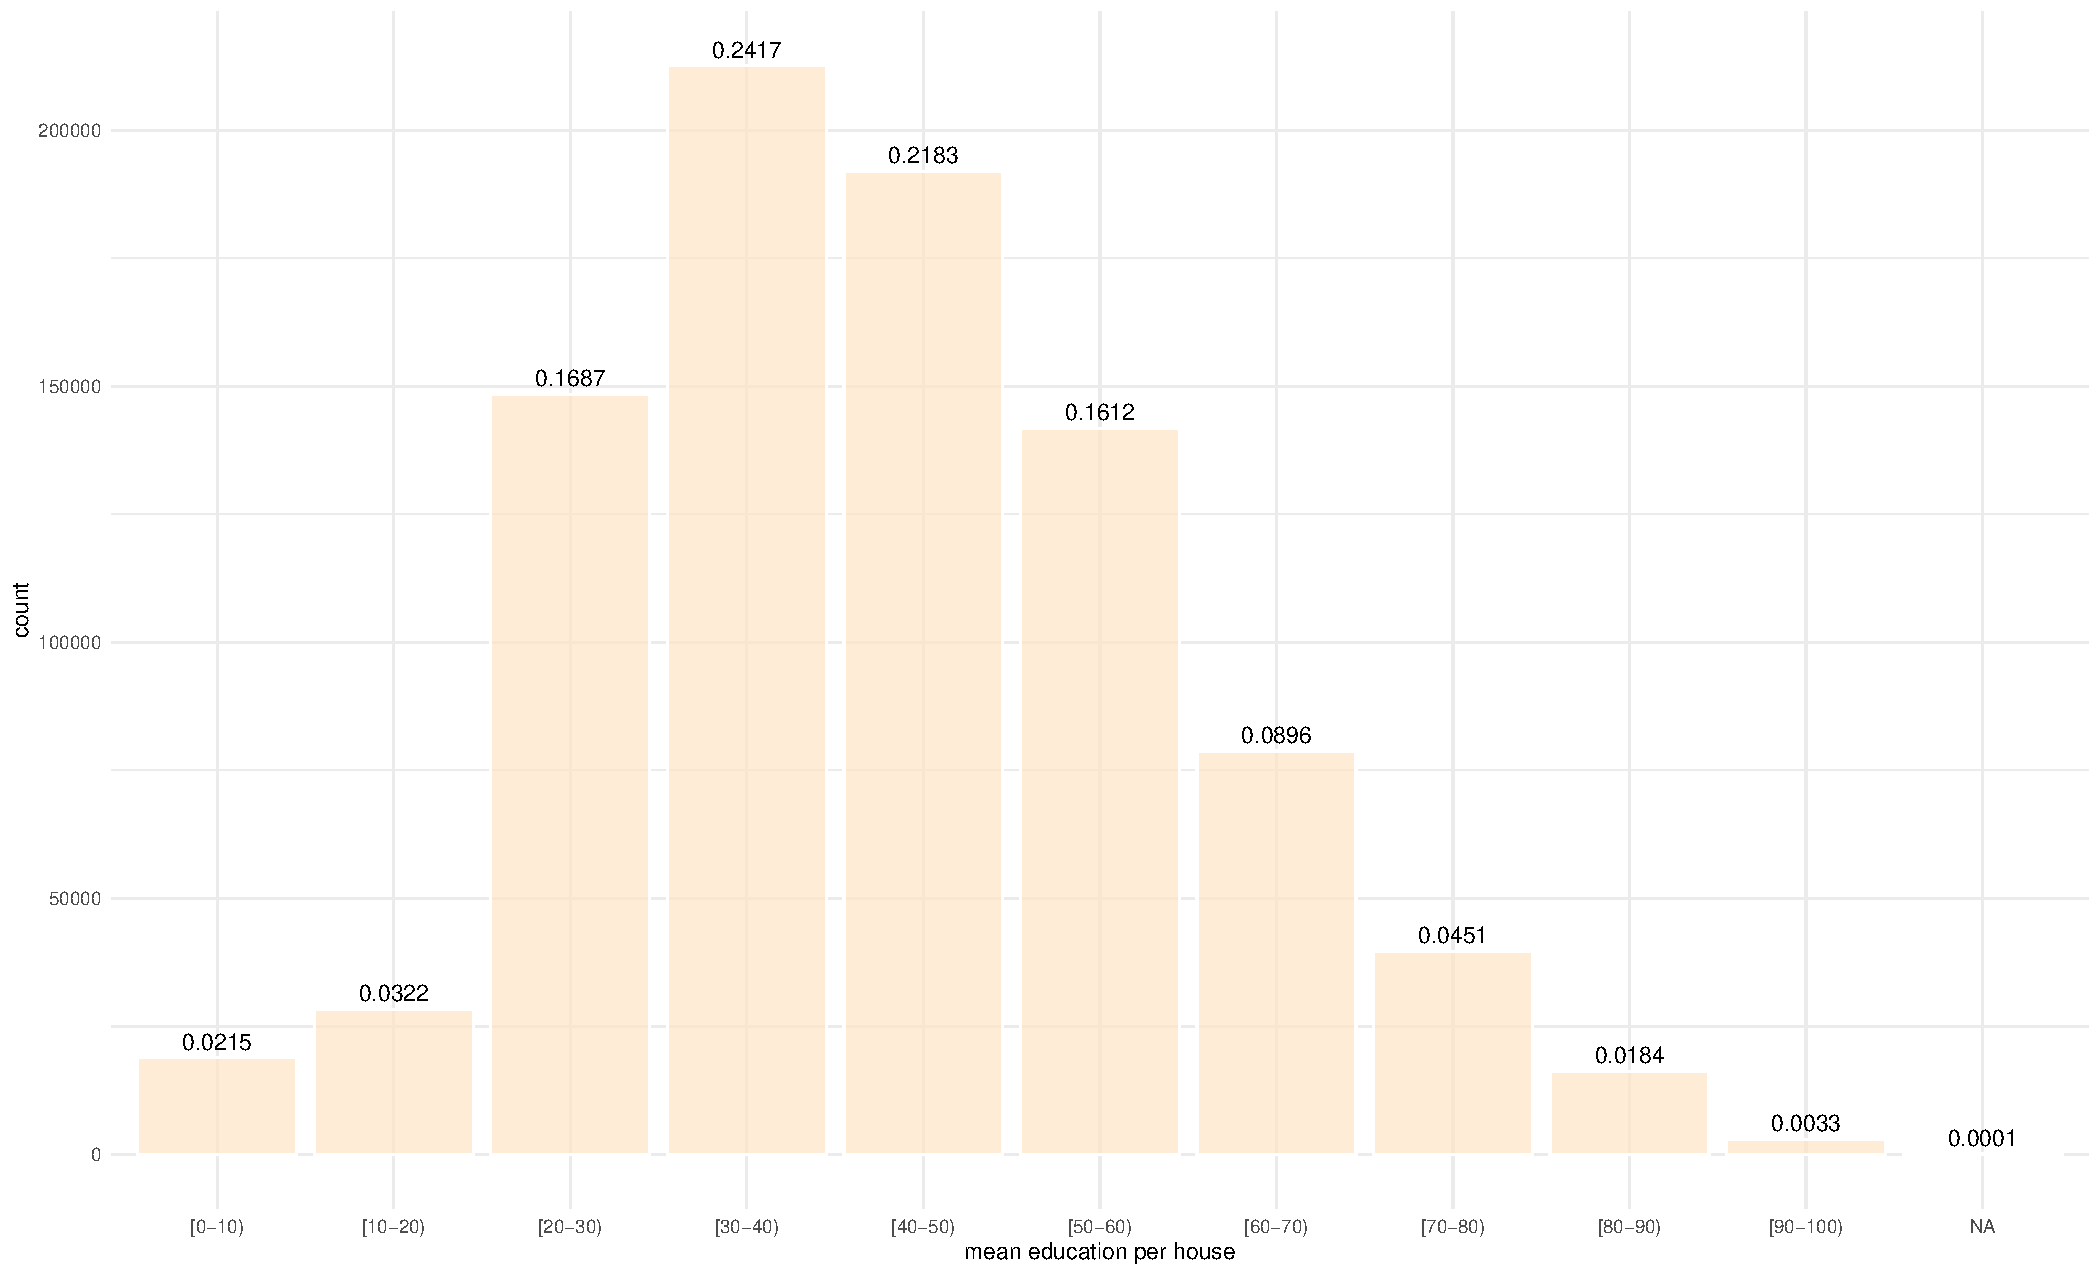
\includegraphics[width=\textwidth]{Rplot02.png}
    \caption{Distribution of cases by age groups in Mexico.}
    \label{fig:LandscapeFigure}
\end{sidewaysfigure}








\bibliographystyle{plainnat}
\bibliography{tarea8}


 
\end{document}